% -*- TeX-master: "/home/joao/DOUTORADO/GIT/Qualificacao/Qualificacao.tex" -*-
%!TEX root = ../Qualificacao.tex

%%%%%%%%%%%%%%%%%%%%%%%%%%%%%%%%%%%%%%%%%%%%%%%%%%%%%%%%%%%%%%%%%%%%%%%
%                 EXAMPLE 4.1 (51) - 2nd Order System                 %
%%%%%%%%%%%%%%%%%%%%%%%%%%%%%%%%%%%%%%%%%%%%%%%%%%%%%%%%%%%%%%%%%%%%%%%


% exemplo 51
\begin{exmp}[Second order Linear System -- continued.]\label{ex:sis2aord}

  Consider the 2nd-order linear system describe in Example \ref{exm:31}: 
  \begin{equation}
    \label{eq:sis2aord}
    y_k = a_1y_{k-1} + a_2y_{k-2} + b_1u_{k-1} + b_2u_{k-2}.
  \end{equation}
  % onde, para $i = 1,\ 2$, os termos $a_i$, $b_i$ $\in \R$, representam parâmetros constantes; $u_{k-i}$ e $y_{k-i}$ $\in \R$, os sinais de entrada e saída, respectivamente; e $k$ o índice temporal.
  According to the VRFT strategy (Chapter ~\ref{cap:VRFT}), one must first define a class of allowable controllers $\mathscr{C}$, containing the desired  structure, and define a reference model that expresses the desired close loop system's behavior.

  In this example, we want to analyze the use of the RAmSS algorithm directly, without modifications, in order to find the best structure for a controller designed from the VRFT strategy.
  In order to examine the behavior of the RaMSS Algorithm in finding the best set of regressors, we proceed as follows.

  A feasible reference model is defined, that is, with a relative degree equal to or greater than that of the process. For simplicity, a 1st order model with the same relative degree of the process is chosen, as Example \ref{exm:31}, given by the transfer function
  \begin{equation}
    M(z) = \frac{1-A}{z-A},
    \label{eq:mr_sis2aord}
  \end{equation}
  The parameter adopted here is the same as Exemple \ref{exm:31}, i.e. $A = -T_s/\tau_d = 0.8187$. 
  The ideal controller, represented by an ARX model, will be given by the structure composed of the regressors presented in \eqref{eq:exp31_uk}, represented here by
  \begin{equation}
    \label{eq:exp51_contIdeal}
    u_k = \theta_0e_{k} + \theta_1e_{k-1} + \theta_2e_{k-2} + \theta_3u_{k-1} + \theta_4u_{k-2},
  \end{equation}
  and will have the parameters shown in \eqref{eq:exp31_ideal_parameters}, described here as
  \begin{equation}
    \vtheta^\star= \begin{bmatrix} \theta^\star_0 & \theta^\star_1 & \theta^\star_2 & \theta^\star_3 & \theta^\star_4 \end{bmatrix}^T =  \begin{bmatrix} 0.181 & 0.308 &  0.145 &  0.19 & 0.81 \end{bmatrix}^T.
  \label{eq:ex51_ideal_parameters}
\end{equation}
Using the RaMSS algorithm, as discussed in the section ~\ref{sec:ramss}, the procedure is performed for 2 cases:
\begin{description}
  \item[case A] the universe set $\mathscr{M}$ is taken as all possible 3rd degree non linear models formed by the monomials up to 4 delays for input $\tilde{e}_k$ (virtual error) and output $\tilde{u}_k$ (virtual process input) collected data. No noise is considered in this case.
  \item[case B] the same case as case A, but now with a noise in the output, given by a gaussian distribution, i.e. $\nu \sim \mathcal{N}(\mu,\sigma)$, where $\mu=0$ is the mean, and $\sigma= 0.1$ is the standard deviation adopted. Note that the noise is added in the output, in a way that the model for the process is represented by an output error model (OEM).
\end{description}
The RaMSS procedure is applied to a data set of 700 samples, obtained via the VRFT procedure, in which the VRFT filter is considered to be unitary, i.e. the data is not filtered. The same data set is applied for the 2 cases. At each iteration, 100 candidate models are randomly chosen to be analyzed, using a Bernoulli process. The RIPs are updated in a maximum of 100 iterations, or until they all converge to a margin above 0.9 or below 0.1, i.e. the following stopping criterion is adopted:
\begin{align}
  \textbf{if } \left[iter<iter_{\max}\right] \textbf{ or } \left[\Delta_S < \frac{1}{2} \left(1-\min_{\forall \mu \in \bm{\mu}_k}{ \left| 2\mu -1 \right| }\right)\right] \textbf{ then} \text{, STOP the procedure.}
\label{eq:crit.par}
\end{align}
where $\Delta_S = 0.1$ is the convergence margin, $iter$ is the iteration number and $iter_{\max} = 100$ is the maximum allowed iterations.


Applying the procedure in both cases, the following controllers are obtained, for a specific realization:
\begin{align}
  % Para caso 24:
  \label{eq:ex51CasesAB}
  u_1(k) &= 0.636{u}_1(k-1) + 0.513{u}_1(k-2) + -0.321{u}_1(k-3) + 0.17{u}_1(k-4) \nonumber\\
      &\quad+ 0.181{e}_1(k) + 0.227{e}_1(k-1) + 0.045{e}_1(k-2) + 0.03{e}_1(k-4) \\
  u_2(k) &= 0.737{u}_2(k-1) + 0.242{u}_2(k-2) + -0.329{u}_2(k-3) + 0.32{u}_2(k-4) \nonumber\\
         &+ 0.175{e}_2(k) + 0.197{e}_2(k-1) + 0.049{e}_2(k-2) + 0.049{e}_2(k-3) + 0.059{e}_2(k-4)
  % u_1(k) &= 0.193{u}_1(k-1) + 0.805{u}_1(k-2)  \nonumber \\
         % &\quad + 0.001{u}_1(k-3) + 0.181{e}_1(k) + 0.307{e}_1(k-1) + 0.144{e}_1(k-2) \nonumber \\
  % u_2(k) &= 0.737{u}_2(k-1) + 0.242{u}_2(k-2) + -0.329{u}_2(k-3) + 0.32{u}_2(k-4)  \\
         % &\quad + 0.175{e}_2(k) + 0.  97{e}_2(k-1) + 0.049{e}_2(k-2) + 0.049{e}_2(k-3) + 0.059{e}_2(k-4)  \nonumber
  % u_1(k) &= 0.193{u}_1(k-1) + 0.805{u}_1(k-2) + 0.001{u}_1(k-3) \\
         % &+ 0.181{e}_1(k) + 0.307{e}_1(k-1) + 0.1441{e}(k-2), \\
  % u_2(k) &= 0.751{u}_2(k-1) + 0.241{u}_2(k-2) -0.33{u}_2(k-3) + 0.322{u}_2(k-4) \\
         % &+ 0.174{e}_2(k) + 0.197{e}_2(k-1) + 0.048{e}_2(k-2) + 0.049{e}_2(k-3) + 0.0591,
\end{align}
where the index subscribed to the variables represent the respective cases.

The table ~\ref{tab:exp51_param} sumarizes the simulation parameters used in \ref{alg:RaMSS}, for the 2 cases,
where $o$ is the maximum allowed degree for the regressors, $n_{\tilde{e}}$ is the maximum delay for the virtual error signal $\tilde{e}(k)$, $n_{\tilde{u}}$ is the maximum delay for the input signal of the sampled plant, $ N_p$ is the number of models chosen at each update of the RIPs, $ iter_{\max} $ is the maximum number of allowed iterations, $\Delta_S$ is the trashold for convergence of RIPs, $K$ is the gain for the performance indexes presented in \ref{eq:Js}, $\gamma_0$ is the initial gain of \ref{eq:gamma}, $\mu_{\min}$ and $\mu_{\max}$ are the minumum and maximum values allowed for the RIPs and $\nu$ is the noise added to the output.
\begin{table}[htpb]
  \centering
  \caption{Parameters for simulating the RaMSS algorithm of the example ~\ref{ex:sis2aord}}\label{tab:exp51_param}
  \begin{tabular}{c|c|c|c|c|c|c|c|c|c|c}
    Case & $o$ & $n_{\tilde{e}}$ & $n_{\tilde{u}}$ & $ N_p$ & $ iter_{\max} $ & $K$ & $\gamma_0$ &  $\mu_{\min}$ & $\mu_{\max}$ & $\nu$\\
    \hline
    A & $ 3 $ & $4$ & $4$ & $100$ & $100$ & $1$ & $2$ & $0.05$ & $1$ & $0$ \\
    B & $ 3 $ & $4$ & $4$ & $100$ & $100$ & $1$ & $2$ & $0.05$ & $1$ & $\mathcal{N}(\mu,\sigma)$
  \end{tabular}
\end{table}\\
\todo[inline]{MEXER NESTA TABELA AINDA! Valores estão errados. Já os modifiquei. Definir parâmetros, etc. Colocar os mais essenciais por aqui e os menos, no appendice. }

Note that the controllers presented in \eqref{eq:ex51CasesAB} are obtained for a specific realization of the procedure. All terms that end with the RIP above 0.95 are considered in the hundredth iteration.
Figure \ref{fig:ex51_RIPevol_2cases} shows the evolution of the RIPs for this realization.

\begin{figure}[H]
  \centering
  % 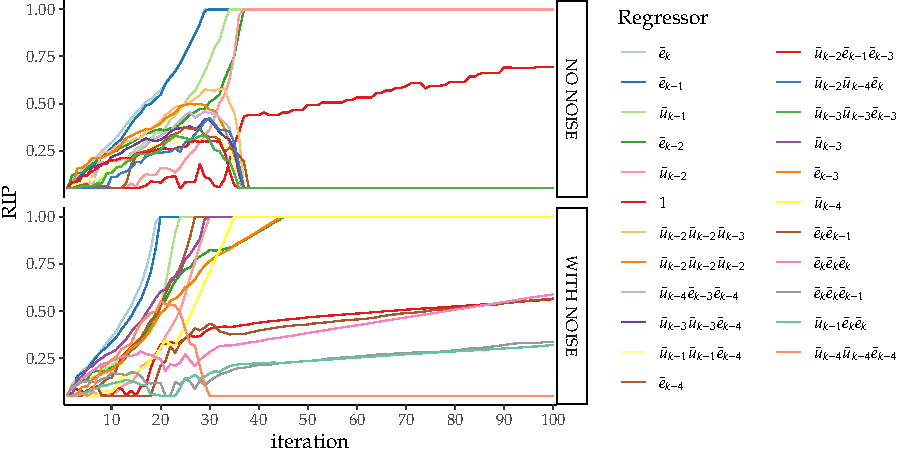
\includegraphics[width=\textwidth]{Figs/Cap5/ex51_rips_evol_2cases.tex.pdf}
  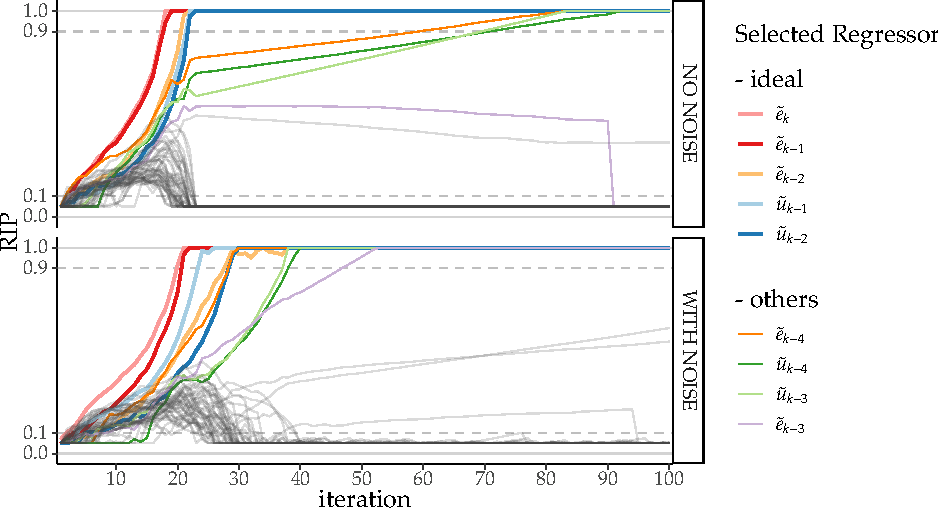
\includegraphics[width=\textwidth]{Figs/Cap5/ex51_rips.tex.pdf}
  \caption{Typical evolution of RIPs for choosing regressors for case 1 and 2.}
  \label{fig:ex51_RIPevol_2cases}
\end{figure}
\todo[inline]{Trocar esta figura} 

The ideal regressors are selected before the first 40 steps.
But as the iterations continue, the $\tilde{u}(k-3)$, $\tilde{u}(k-4)$ and $\tilde{e}(k-4)$ regressors continue to increase monotonically in value and eventually end up being selected.
The effect of including these terms, although in general they are small, deteriorates the desired behavior of the controller.
When considering noise in the measurement (case 2), the selection of non-ideal regressors occurs even earlier, as can be seen in the lower graph of \ref{fig:ex51_RIPevol_2cases}.
Part of this result is due to the worsening of parametric identification during the VRFT procedure, provoked by the polarization effect introduced by noise at the output. The result is that the regressor vectors are no longer orthogonal to the residuals and the OLS estimator becomes polarized. A strategy to mitigate this effect is to use non-polarized estimators, such as VI estimators, or even the ELS.

Figure ~\ref{fig:Figs-RespostaSist2aordNARX-png} shows the temporal response for the controllers identified in \eqref{eq:ex51CasesAB}, when the reference signal is taken as a square wave.

% The figure  shows the temporal response for a square wave in reference signal, for the 2 cases.
% Note que no Caso 1,

\begin{figure}[H]
  \sbox0{\blacksolidlinethin} \sbox1{\bluedashedline} \sbox2{\reddottedline} \sbox3{\blackdottedline} \sbox4{\bluedashdotedline} 
  \centering
  % 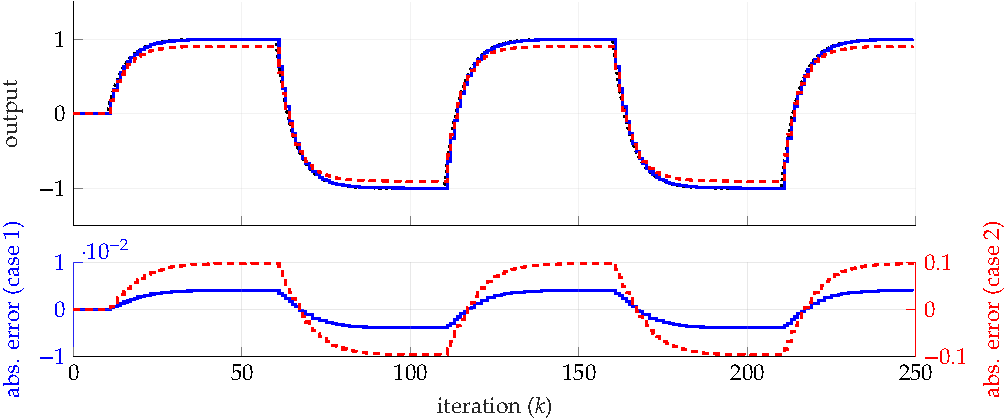
\includegraphics[width=1\textwidth]{./Figs/Cap5/ex51_resp_temporal_mf_editado.tex.pdf}
  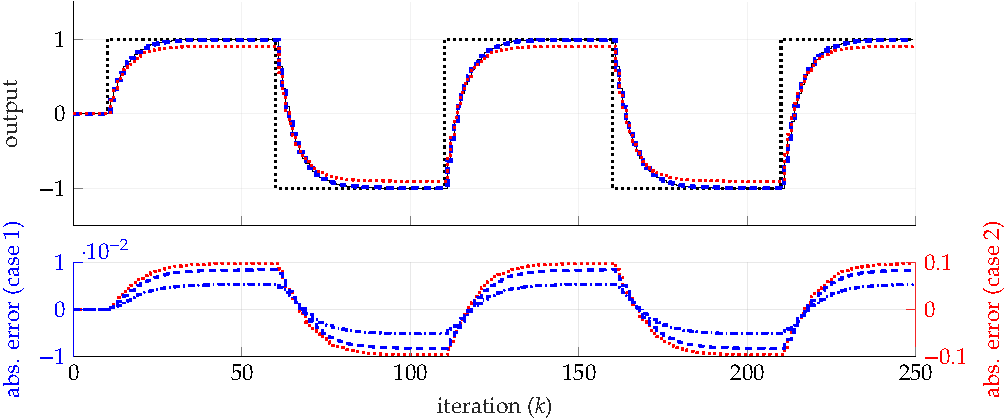
\includegraphics[width=1\textwidth]{./Figs/Cap5/ex51_resp_temporal_mf2.tex.pdf}
  % % This file was created by matlab2tikz.
%
%The latest updates can be retrieved from
%  http://www.mathworks.com/matlabcentral/fileexchange/22022-matlab2tikz-matlab2tikz
%where you can also make suggestions and rate matlab2tikz.
%
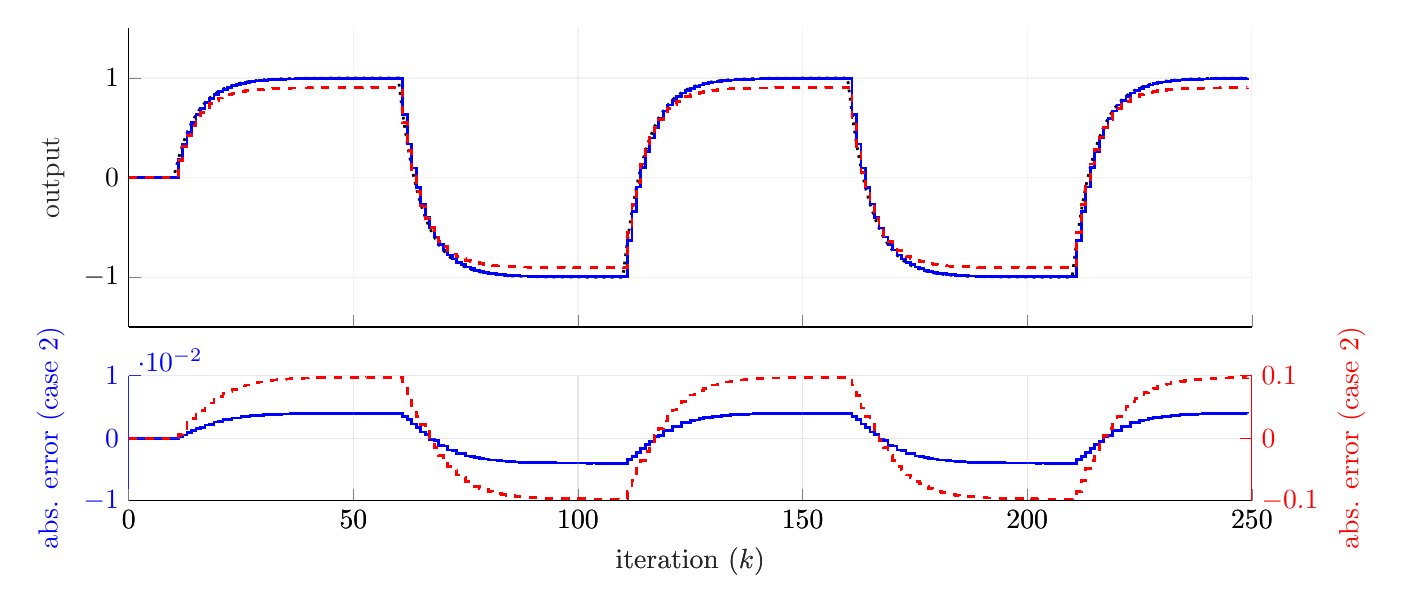
\begin{tikzpicture}

\begin{axis}[%
width=14.264cm,
height=3.794cm,
at={(0cm,2.206cm)},
scale only axis,
xmin=0,
xmax=250,
xtick={0,50,100,150,200,250},
xticklabels={{},{},{},{},{},{}},
ymin=-1.5,
ymax=1.5,
ylabel style={font=\color{white!15!black}},
ylabel={output},
axis background/.style={fill=white},
axis x line*=bottom,
axis y line*=left,
xmajorgrids,
ymajorgrids,
grid style={opacity=0.2}
]
\addplot [color=black, dotted, line width=1.0pt, forget plot]
  table[row sep=crcr]{%
0	0\\
10	0\\
11	0.181269246922028\\
12	0.329679953964359\\
13	0.45118836390597\\
14	0.550671035882772\\
15	0.632120558828547\\
16	0.69880578808781\\
17	0.753403036058387\\
18	0.798103482005331\\
19	0.834701111778401\\
20	0.8646647167634\\
21	0.88919684163767\\
22	0.909282046710587\\
23	0.925726421785669\\
24	0.939189937374778\\
25	0.950212931632137\\
26	0.959237796021625\\
27	0.966626730039678\\
28	0.972676277552694\\
30	0.981684361111263\\
32	0.987722660096921\\
34	0.991770252950971\\
37	0.995483419057393\\
41	0.997970569363702\\
47	0.999388747238868\\
60	0.999954600070225\\
61	0.637424335837267\\
62	0.340609659588267\\
63	0.0975983561783096\\
64	-0.10136247126897\\
65	-0.264257819357908\\
66	-0.397625250371675\\
67	-0.506817267601633\\
68	-0.596216130098412\\
69	-0.669409728114744\\
70	-0.729335577739135\\
71	-0.778398713730951\\
72	-0.818568212009893\\
73	-0.85145621558658\\
74	-0.878382635522144\\
75	-0.900428123593684\\
76	-0.918477442644473\\
77	-0.933254975223463\\
78	-0.945353795600482\\
79	-0.955259471919135\\
80	-0.963369553751249\\
81	-0.970009527157174\\
82	-0.975445877584235\\
84	-0.983540879531887\\
86	-0.988967121610102\\
88	-0.992604440449782\\
91	-0.995941230863423\\
95	-0.998176277468275\\
102	-0.999550275560608\\
110	-0.999909202201621\\
111	-0.637387167206128\\
112	-0.340579228486888\\
113	-0.0975734412997724\\
114	0.101382869846248\\
115	0.264274520300432\\
116	0.397638923946914\\
117	0.506828462578198\\
118	0.596225295770012\\
119	0.669417232331938\\
120	0.72934172167254\\
121	0.778403743958165\\
122	0.818572330411598\\
123	0.851459587448716\\
124	0.878385396169364\\
125	0.900430383820463\\
126	0.918479293161653\\
127	0.933256490298788\\
128	0.945355036039246\\
129	0.955260487504489\\
130	0.963370385242229\\
131	0.970010207924418\\
132	0.975446434949305\\
134	0.983541253144864\\
136	0.988967372050382\\
138	0.99260460832491\\
141	0.995941322995236\\
145	0.998176318865774\\
152	0.999550285769089\\
160	0.999909204262678\\
161	0.637387168893582\\
162	0.340579229868467\\
163	0.0975734424308996\\
164	-0.101382868920155\\
165	-0.264274519542226\\
166	-0.397638923326127\\
167	-0.506828462069933\\
168	-0.596225295353889\\
169	-0.669417231991247\\
170	-0.72934172139361\\
171	-0.778403743729797\\
172	-0.81857233022464\\
173	-0.851459587295636\\
174	-0.878385396044024\\
175	-0.900430383717861\\
176	-0.918479293077638\\
177	-0.933256490230008\\
178	-0.945355035982942\\
179	-0.955260487458389\\
180	-0.963370385204456\\
181	-0.970010207893495\\
182	-0.975446434923981\\
184	-0.983541253127925\\
186	-0.988967372039014\\
188	-0.992604608317293\\
191	-0.995941322991058\\
195	-0.998176318863898\\
202	-0.999550285768635\\
210	-0.999909204262593\\
211	-0.637387168893497\\
212	-0.34057922986841\\
213	-0.0975734424308712\\
214	0.101382868920183\\
215	0.264274519542255\\
216	0.397638923326156\\
217	0.506828462069961\\
218	0.596225295353918\\
219	0.669417231991275\\
220	0.72934172139361\\
221	0.778403743729797\\
222	0.81857233022464\\
223	0.851459587295636\\
224	0.878385396044052\\
225	0.900430383717861\\
226	0.918479293077638\\
227	0.933256490230008\\
228	0.945355035982942\\
229	0.955260487458389\\
230	0.963370385204485\\
231	0.970010207893495\\
232	0.975446434923981\\
234	0.983541253127925\\
236	0.988967372039014\\
238	0.992604608317293\\
241	0.995941322991058\\
245	0.998176318863898\\
249	0.999180567244224\\
};
\addplot[const plot, color=blue, line width=1.0pt, forget plot] table[row sep=crcr] {%
0	0\\
11	0.180977171837526\\
12	0.329172712212909\\
13	0.45031150992321\\
14	0.54950721174589\\
15	0.630603534262377\\
16	0.697071838198383\\
17	0.75129926836172\\
18	0.795887192211239\\
19	0.832113918402939\\
20	0.862042313411223\\
21	0.886239644815532\\
22	0.906320094899854\\
23	0.922499135273426\\
24	0.935950021055618\\
25	0.946791840399243\\
26	0.955778629339733\\
27	0.963064221517527\\
28	0.969052500940336\\
29	0.973959104837405\\
30	0.977943604763652\\
31	0.981248875948808\\
32	0.983902902127539\\
33	0.986123664527099\\
34	0.987898809353766\\
35	0.98938291118904\\
36	0.990577874726654\\
37	0.991563033579666\\
38	0.99237257824521\\
39	0.99302302327095\\
40	0.993573142885879\\
41	0.994002292764549\\
42	0.994375004464132\\
43	0.994660023006162\\
44	0.99491004110115\\
45	0.995101960911995\\
46	0.995267159859196\\
47	0.995398551232711\\
48	0.995506018603493\\
49	0.995597031866481\\
50	0.995666340606363\\
51	0.995729353060426\\
52	0.995774354984661\\
53	0.995817277218976\\
54	0.995847290647959\\
55	0.995875646946359\\
56	0.995896489317232\\
57	0.995914513739081\\
58	0.99592950784691\\
59	0.995940580406312\\
60	0.995951482435515\\
61	0.634003883369871\\
62	0.337620550089099\\
63	0.0953472448544233\\
64	-0.10303894571345\\
65	-0.2652285809788\\
66	-0.39816195207419\\
67	-0.506614475468581\\
68	-0.595788499822845\\
69	-0.668240060126379\\
70	-0.728095910664535\\
71	-0.776489090096334\\
72	-0.816649504165156\\
73	-0.849006521870962\\
74	-0.875907972279464\\
75	-0.897590947700024\\
76	-0.915564224598512\\
77	-0.930135072159629\\
78	-0.942111315794165\\
79	-0.951924405502382\\
80	-0.959893102619901\\
81	-0.966503635844077\\
82	-0.971811439975454\\
83	-0.976252980102885\\
84	-0.979803103504366\\
85	-0.982771300351828\\
86	-0.985161145199214\\
87	-0.987131422548657\\
88	-0.98875049439485\\
89	-0.990051322178317\\
90	-0.99115157956436\\
91	-0.992009815056377\\
92	-0.992755265095326\\
93	-0.993325252586487\\
94	-0.993825306183027\\
95	-0.994209118582432\\
96	-0.994539518302446\\
97	-0.994802294746677\\
98	-0.995017218301086\\
99	-0.995199252164724\\
100	-0.995337852432442\\
101	-0.995463889534307\\
102	-0.995553877257976\\
103	-0.995639731886712\\
104	-0.995699748235978\\
105	-0.995756465549192\\
106	-0.995798146571843\\
107	-0.995834194602935\\
108	-0.995864184425045\\
109	-0.995886325211501\\
110	-0.995908133508522\\
111	-0.633967273804899\\
112	-0.337591692291056\\
113	-0.0953226731259633\\
114	0.103058301629801\\
115	0.265244929159081\\
116	0.398175062764892\\
117	0.506625249266051\\
118	0.595797451149849\\
119	0.668247118158689\\
120	0.728102030832304\\
121	0.776493725318176\\
122	0.816653654829679\\
123	0.84900960826289\\
124	0.875910738485828\\
125	0.897593050066035\\
126	0.915566026255306\\
127	0.930136537077203\\
128	0.942112465237926\\
129	0.951925437303544\\
130	0.959893831175947\\
131	0.966504355793973\\
132	0.971811911211717\\
133	0.976253467082586\\
134	0.979803423931486\\
135	0.982771614147225\\
136	0.985161376691991\\
137	0.987131613667088\\
138	0.988750668125164\\
139	0.990051433495751\\
140	0.991151709211351\\
141	0.992009880262856\\
142	0.992755357103761\\
143	0.993325294868953\\
144	0.993825365970537\\
145	0.994209151088342\\
146	0.994539552657386\\
147	0.994802322807573\\
148	0.995017235142114\\
149	0.995199276392725\\
150	0.99533785939127\\
151	0.995463908745052\\
152	0.995553880291141\\
153	0.995639745123498\\
154	0.995699750932573\\
155	0.995756472981157\\
156	0.995798150277864\\
157	0.99583419749294\\
158	0.995864188932899\\
159	0.995886325370492\\
160	0.99590813792517\\
161	0.633967272955033\\
162	0.337591695755407\\
163	0.0953226724599574\\
164	-0.103058299551094\\
165	-0.265244929117785\\
166	-0.398175062008676\\
167	-0.506625248547522\\
168	-0.595797451309551\\
169	-0.668247117097962\\
170	-0.728102031391813\\
171	-0.776493724302242\\
172	-0.816653655361904\\
173	-0.849009607559282\\
174	-0.875910738755806\\
175	-0.89759304976053\\
176	-0.915566026223672\\
177	-0.930136537101305\\
178	-0.942112464997905\\
179	-0.951925437508748\\
180	-0.959893830868879\\
181	-0.966504356028963\\
182	-0.971811910957314\\
183	-0.976253467244817\\
184	-0.979803423791878\\
185	-0.982771614199692\\
186	-0.985161376669453\\
187	-0.987131613626559\\
188	-0.988750668181922\\
189	-0.99005143340699\\
190	-0.991151709296645\\
191	-0.992009880172304\\
192	-0.992755357175952\\
193	-0.993325294807619\\
194	-0.993825366007997\\
195	-0.994209151066315\\
196	-0.994539552658807\\
197	-0.994802322817804\\
198	-0.995017235119491\\
199	-0.995199276419669\\
200	-0.995337859360859\\
201	-0.99546390877299\\
202	-0.995553880266129\\
203	-0.995639745142142\\
204	-0.99569975091967\\
205	-0.995756472987182\\
206	-0.995798150277125\\
207	-0.995834197488733\\
208	-0.995864188940118\\
209	-0.995886325361141\\
210	-0.995908137934919\\
211	-0.633967272945597\\
212	-0.337591695763365\\
213	-0.0953226724537615\\
214	0.103058299547115\\
215	0.265244929119746\\
216	0.398175062008619\\
217	0.506625248546129\\
218	0.59579745131208\\
219	0.668247117094865\\
220	0.728102031395082\\
221	0.7764937242992\\
222	0.816653655364519\\
223	0.849009607557321\\
224	0.875910738757113\\
225	0.897593049759934\\
226	0.915566026223644\\
227	0.930136537101816\\
228	0.942112464997081\\
229	0.951925437509772\\
230	0.959893830867799\\
231	0.966504356029986\\
232	0.971811910956461\\
233	0.976253467245471\\
234	0.979803423791452\\
235	0.982771614199862\\
236	0.985161376669453\\
237	0.987131613626389\\
238	0.988750668182206\\
239	0.990051433406649\\
240	0.991151709297014\\
241	0.992009880171963\\
242	0.992755357176208\\
243	0.99332529480742\\
244	0.993825366008139\\
245	0.994209151066258\\
246	0.994539552658807\\
247	0.99480232281789\\
248	0.995017235119377\\
249	0.995199276419783\\
};
\addplot[const plot, color=red, dashed, line width=1.0pt, forget plot] table[row sep=crcr] {%
0	0\\
11	0.175057837660773\\
12	0.315108606907074\\
13	0.426588150709449\\
14	0.51956167119738\\
15	0.594286109260821\\
16	0.655135784739997\\
17	0.702527697924609\\
18	0.741838777618398\\
19	0.77225983010905\\
20	0.798373587886005\\
21	0.817964067832179\\
22	0.8350736083475\\
23	0.847611071714567\\
24	0.858723810104294\\
25	0.866922466539478\\
26	0.874060824457501\\
27	0.879513082557196\\
28	0.883999242995742\\
29	0.887673652014797\\
30	0.890462181039311\\
31	0.892949013964\\
32	0.894689964971832\\
33	0.896343978862291\\
34	0.897461842614717\\
35	0.898523537010391\\
36	0.899278919205585\\
37	0.899927562215879\\
38	0.900463534863803\\
39	0.90083967915939\\
40	0.901227428975886\\
41	0.90143979655096\\
42	0.901713732305325\\
43	0.901839323230234\\
44	0.902020253342215\\
45	0.902106347904407\\
46	0.902213540384309\\
47	0.902283235255084\\
48	0.902337553824992\\
49	0.902397723252136\\
50	0.902419819972835\\
51	0.902469326037533\\
52	0.902476441913677\\
53	0.902512513076459\\
54	0.90251623038057\\
55	0.902538032212703\\
56	0.902543914642166\\
57	0.902553458871893\\
58	0.902562340116049\\
59	0.90256361457989\\
60	0.902573698170528\\
61	0.552455445478785\\
62	0.272362786933741\\
63	0.0494007823988909\\
64	-0.136540247295017\\
65	-0.285990440390719\\
66	-0.407687067631656\\
67	-0.502470205440403\\
68	-0.581092278701334\\
69	-0.641932311178806\\
70	-0.694161189176867\\
71	-0.733339692463602\\
72	-0.767560412461251\\
73	-0.79263335075575\\
74	-0.814859956970821\\
75	-0.831256182941274\\
76	-0.845533232563184\\
77	-0.856437559375536\\
78	-0.865409538605803\\
79	-0.872758770170918\\
80	-0.878335140896809\\
81	-0.88330943754994\\
82	-0.886790649753493\\
83	-0.890099211291471\\
84	-0.892334474714488\\
85	-0.894458138169568\\
86	-0.895968736547701\\
87	-0.897266028287817\\
88	-0.898338051108368\\
89	-0.899090166389698\\
90	-0.899865869116638\\
91	-0.900290373633823\\
92	-0.900838455599256\\
93	-0.901089448591165\\
94	-0.901451449058101\\
95	-0.901623540769322\\
96	-0.901837971016619\\
97	-0.901977355190809\\
98	-0.902085960258347\\
99	-0.902206353892666\\
100	-0.9022504763999\\
101	-0.90234956258152\\
102	-0.902363722937849\\
103	-0.902435925631892\\
104	-0.902443313274432\\
105	-0.902486947330146\\
106	-0.902498697163736\\
107	-0.902517786090243\\
108	-0.902535559211117\\
109	-0.902538089185128\\
110	-0.90255827970293\\
111	-0.552437424800161\\
112	-0.272353669518367\\
113	-0.0493887280749448\\
114	0.136546275187442\\
115	0.285997795158806\\
116	0.407691694069229\\
117	0.502474143318068\\
118	0.581096134216409\\
119	0.641934087841918\\
120	0.694164336115279\\
121	0.733340374593951\\
122	0.767562741271121\\
123	0.792633684597831\\
124	0.814861425197137\\
125	0.831256561092516\\
126	0.845533945951161\\
127	0.8564380834612\\
128	0.865409719746452\\
129	0.872759366985946\\
130	0.87833504778024\\
131	0.8833099779593\\
132	0.886790497812001\\
133	0.890099595248756\\
134	0.892334392981667\\
135	0.894458332123122\\
136	0.895968764038798\\
137	0.89726606144643\\
138	0.898338162241629\\
139	0.899090103490011\\
140	0.899866010181398\\
141	0.900290283164196\\
142	0.900838576423098\\
143	0.901089379855762\\
144	0.901451521089001\\
145	0.901623515058702\\
146	0.901837990733185\\
147	0.901977369365483\\
148	0.902085942205645\\
149	0.902206390863569\\
150	0.902250442146482\\
151	0.902349602678896\\
152	0.902363691363718\\
153	0.902435954655999\\
154	0.902443295162755\\
155	0.902486959715276\\
156	0.902498694480471\\
157	0.902517783862891\\
158	0.902535567669759\\
159	0.902538078608103\\
160	0.902558292559149\\
161	0.552437412716728\\
162	0.272353680841377\\
163	0.0493887193443356\\
164	-0.136546268713317\\
165	-0.285997798625345\\
166	-0.407691692909395\\
167	-0.502474142154227\\
168	-0.581096136835015\\
169	-0.641934084084795\\
170	-0.694164340221533\\
171	-0.733340370465015\\
172	-0.767562744884572\\
173	-0.792633681658486\\
174	-0.814861427224344\\
175	-0.831256559933763\\
176	-0.845533946247315\\
177	-0.856438083843869\\
178	-0.865409718824651\\
179	-0.872759368220756\\
180	-0.878335046395961\\
181	-0.883309979307967\\
182	-0.886790496612093\\
183	-0.890099596198667\\
184	-0.892334392317451\\
185	-0.894458332484959\\
186	-0.895968763949213\\
187	-0.897266061304208\\
188	-0.898338162551482\\
189	-0.899090103073632\\
190	-0.89986601063913\\
191	-0.900290282716924\\
192	-0.900838576815858\\
193	-0.901089379544487\\
194	-0.901451521302931\\
195	-0.901623514943168\\
196	-0.901837990757684\\
197	-0.901977369415732\\
198	-0.90208594210003\\
199	-0.902206391002636\\
200	-0.90225044199417\\
201	-0.902349602826376\\
202	-0.902363691234569\\
203	-0.902435954757436\\
204	-0.902443295093491\\
205	-0.902486959751769\\
206	-0.902498694473763\\
207	-0.902517783844985\\
208	-0.902535567705542\\
209	-0.902538078561548\\
210	-0.902558292609712\\
211	-0.552437412668013\\
212	-0.272353680883754\\
213	-0.0493887193112243\\
214	0.13654626869095\\
215	0.285997798636885\\
216	0.40769169290769\\
217	0.502474142147918\\
218	0.581096136847151\\
219	0.64193408406922\\
220	0.694164340238331\\
221	0.733340370448957\\
222	0.76756274489847\\
223	0.792633681647686\\
224	0.814861427231563\\
225	0.831256559930125\\
226	0.845533946247713\\
227	0.856438083846086\\
228	0.865409718820558\\
229	0.872759368225985\\
230	0.87833504639039\\
231	0.883309979313253\\
232	0.886790496607517\\
233	0.890099596202163\\
234	0.892334392315121\\
235	0.894458332486096\\
236	0.895968763949128\\
237	0.897266061303441\\
238	0.898338162552875\\
239	0.899090103071899\\
240	0.899866010640977\\
241	0.90029028271519\\
242	0.900838576817335\\
243	0.90108937954335\\
244	0.901451521303699\\
245	0.901623514942827\\
246	0.901837990757713\\
247	0.901977369416016\\
248	0.902085942099575\\
249	0.902206391003205\\
};
\end{axis}

\begin{axis}[%
width=14.264cm,
height=1.588cm,
at={(0cm,0cm)},
scale only axis,
xmin=0,
xmax=250,
xtick={  0,  50, 100, 150, 200, 250},
xlabel style={font=\color{white!15!black}},
xlabel={iteration ($k$)},
every outer y axis line/.append style={blue},
every y tick label/.append style={font=\color{blue}},
every y tick/.append style={blue},
ymin=-0.01,
ymax=0.01,
ytick={-0.01,    0,  0.01},
ylabel style={font=\color{blue}},
ylabel={abs. error (case 2)},
axis background/.style={fill=white},
axis x line*=bottom,
axis y line*=left,
xmajorgrids,
ymajorgrids,
grid style={opacity=0.2}
]
\addplot[const plot, color=blue, line width=1.0pt, forget plot] table[row sep=crcr] {%
0	0\\
1	0\\
2	0\\
3	0\\
4	0\\
5	0\\
6	0\\
7	0\\
8	0\\
9	0\\
10	0\\
11	0.000292075084480176\\
12	0.000507241751442511\\
13	0.000876853982768211\\
14	0.00116382413687421\\
15	0.00151702456619074\\
16	0.00173394988941156\\
17	0.00210376769667719\\
18	0.00221628979410016\\
19	0.00258719337547819\\
20	0.00262240335216601\\
21	0.00295719682212836\\
22	0.00296195181074288\\
23	0.00322728651224391\\
24	0.00323991631917342\\
25	0.00342109123288703\\
26	0.00345916668188717\\
27	0.00356250852214923\\
28	0.00362377661237734\\
29	0.00367012330641792\\
30	0.00374075634761539\\
31	0.00375554723070715\\
32	0.0038197579694017\\
33	0.00382449972826293\\
34	0.00387144359722236\\
35	0.00387914181186799\\
36	0.00390556085257976\\
37	0.003920385477724\\
38	0.00392955803829997\\
39	0.00394942198368098\\
40	0.00394810493746622\\
41	0.00396827659916044\\
42	0.00396343826270495\\
43	0.00397960895628502\\
44	0.00397618375101072\\
45	0.00398615712244876\\
46	0.00398625433243327\\
47	0.00399019600617267\\
48	0.00399352996306945\\
49	0.00399323315453592\\
50	0.00399819676572899\\
51	0.00399599336960055\\
52	0.00400077769115237\\
53	0.00399861698736281\\
54	0.00400197627695031\\
55	0.00400094324955269\\
56	0.00400247128091957\\
57	0.00400276219535611\\
58	0.00400276341660322\\
59	0.00400396799425162\\
60	0.00400311763472017\\
61	0.00342045246740397\\
62	0.00298910949916176\\
63	0.00225111132390626\\
64	0.00167647444448767\\
65	0.000970761620900262\\
66	0.00053670170253789\\
67	-0.000202792133058294\\
68	-0.000427630275575797\\
69	-0.00116966798834894\\
70	-0.00123966707460521\\
71	-0.00190962363459402\\
72	-0.0019187078447348\\
73	-0.00244969371561099\\
74	-0.00247466324267154\\
75	-0.00283717589365973\\
76	-0.00291321804596179\\
77	-0.00311990306384202\\
78	-0.00324247980633918\\
79	-0.00333506641676307\\
80	-0.00347645113133588\\
81	-0.00350589131308976\\
82	-0.00363443760877347\\
83	-0.00364380476048398\\
84	-0.00373777602751957\\
85	-0.00375311155233304\\
86	-0.00380597641089231\\
87	-0.0038356206185729\\
88	-0.00385394605493539\\
89	-0.00389370578169757\\
90	-0.0038910286174958\\
91	-0.00393141580705081\\
92	-0.00392169579289658\\
93	-0.00395407309902984\\
94	-0.00394719408658994\\
95	-0.00396715888583332\\
96	-0.00396734397573517\\
97	-0.00397522748190737\\
98	-0.00398190155247902\\
99	-0.00398129647926482\\
100	-0.00399123754172281\\
101	-0.00398681579500204\\
102	-0.0039963983026271\\
103	-0.00399206488434289\\
104	-0.00399879245710966\\
105	-0.00399672044542354\\
106	-0.00399977921166095\\
107	-0.00400036102161183\\
108	-0.00400036117686398\\
109	-0.00400277410712702\\
110	-0.00400106869311345\\
111	-0.00341989340122295\\
112	-0.00298753619584657\\
113	-0.00225076817381159\\
114	-0.00167543178356248\\
115	-0.000970408858629701\\
116	-0.00053613881796849\\
117	0.000203213312159445\\
118	0.000427844620166873\\
119	0.0011701141732714\\
120	0.00123969084024012\\
121	0.00191001863999063\\
122	0.00191867558193748\\
123	0.00244997918583401\\
124	0.00247465768353172\\
125	0.00283733375442097\\
126	0.00291326690633198\\
127	0.00311995322157321\\
128	0.00324257080133794\\
129	0.0033350502009688\\
130	0.00347655406626723\\
131	0.00350585213043086\\
132	0.00363452373757811\\
133	0.00364377411269301\\
134	0.00373782921340127\\
135	0.00375310364534343\\
136	0.00380599535839243\\
137	0.00383563454330016\\
138	0.00385394019975016\\
139	0.00389373190879105\\
140	0.00389101150056026\\
141	0.00393144273239565\\
142	0.00392167921562592\\
143	0.00395409257437607\\
144	0.00394718486209822\\
145	0.00396716777743467\\
146	0.00396734351420325\\
147	0.00397522717058285\\
148	0.003981907430891\\
149	0.00398129085234122\\
150	0.00399124581218158\\
151	0.00398680905295301\\
152	0.00399640547796387\\
153	0.00399206000556518\\
154	0.00399879660345326\\
155	0.00399671861602235\\
156	0.00399978009260493\\
157	0.00400036188710118\\
158	0.00400035974375212\\
159	0.00400277646552949\\
160	0.00400106633752628\\
161	0.00341989593855241\\
162	0.00298753411306452\\
163	0.00225076997095258\\
164	0.0016754306309507\\
165	0.000970409575570597\\
166	0.000536138682531273\\
167	-0.000203213522417256\\
168	-0.000427844044339598\\
169	-0.00117011489330998\\
170	-0.0012396900017928\\
171	-0.00191001942753999\\
172	-0.00191867486272546\\
173	-0.0024499797363432\\
174	-0.00247465728822305\\
175	-0.002837333957323\\
176	-0.00291326685396387\\
177	-0.00311995312869495\\
178	-0.00324257098502245\\
179	-0.00333504994965905\\
180	-0.00347655433559468\\
181	-0.00350585186453212\\
182	-0.00363452396668873\\
183	-0.00364377392974446\\
184	-0.0037378293360445\\
185	-0.00375310357901482\\
186	-0.00380599536957138\\
187	-0.00383563457451486\\
188	-0.00385394013537876\\
189	-0.00389373199132259\\
190	-0.00389101141014303\\
191	-0.00393144281876945\\
192	-0.00392167914002972\\
193	-0.00395409263289803\\
194	-0.00394718482234657\\
195	-0.00396716779758555\\
196	-0.00396734351124772\\
197	-0.00397522715906962\\
198	-0.00398190745249094\\
199	-0.00398129082454735\\
200	-0.00399124584192367\\
201	-0.00398680902443249\\
202	-0.00399640550249958\\
203	-0.00399205998653973\\
204	-0.00399879661606162\\
205	-0.00399671860972017\\
206	-0.00399978009315893\\
207	-0.00400036189114261\\
208	-0.00400035973638824\\
209	-0.00400277647477565\\
210	-0.00400106632766373\\
211	-0.00341989594789505\\
212	-0.00298753410504804\\
213	-0.00225076997708706\\
214	-0.00167543062691854\\
215	-0.000970409577503994\\
216	-0.000536138682459331\\
217	0.00020321352385122\\
218	0.000427844041851144\\
219	0.00117011489639962\\
220	0.0012396899985363\\
221	0.00191001943060864\\
222	0.00191867486011654\\
223	0.00244997973832595\\
224	0.00247465728694085\\
225	0.00283733395791852\\
226	0.00291326685397897\\
227	0.00311995312819424\\
228	0.00324257098586322\\
229	0.0033350499486311\\
230	0.0034765543366706\\
231	0.00350585186352603\\
232	0.00363452396753938\\
233	0.00364377392910298\\
234	0.00373782933645517\\
235	0.00375310357882996\\
236	0.00380599536955673\\
237	0.00383563457468727\\
238	0.00385394013509677\\
239	0.00389373199166376\\
240	0.00389101140978809\\
241	0.00393144281909896\\
242	0.00392167913975283\\
243	0.00395409263310453\\
244	0.00394718482221668\\
245	0.00396716779764061\\
246	0.00396734351125749\\
247	0.00397522715900855\\
248	0.00398190745258664\\
249	0.00398129082443366\\
};
\end{axis}

\begin{axis}[%
width=14.264cm,
height=1.588cm,
at={(0cm,0cm)},
scale only axis,
xmin=0,
xmax=250,
xtick={  0,  50, 100, 150, 200, 250},
xlabel style={font=\color{white!15!black}},
xlabel={iteration ($k$)},
every outer y axis line/.append style={red},
every y tick label/.append style={font=\color{red}},
every y tick/.append style={red},
ymin=-0.1,
ymax=0.1,
ytick={-0.1,    0,  0.1},
ylabel style={font=\color{red}},
ylabel={abs. error (case 2)},
axis background/.style={fill=none},
axis x line*=bottom,
axis y line*=right,
xmajorgrids,
ymajorgrids,
grid style={opacity=0.2}
]
\addplot[const plot, color=red, dashed, line width=1.0pt, forget plot] table[row sep=crcr] {%
0	0\\
11	0.00621140926125463\\
12	0.0145713470572844\\
13	0.0246002131965213\\
14	0.0311093646853919\\
15	0.0378344495677254\\
16	0.0436700033477848\\
17	0.0508753381337783\\
18	0.0562647043869333\\
19	0.0624412816693507\\
20	0.0662911288773955\\
21	0.071232773805491\\
22	0.0742084383630868\\
23	0.0781153500711014\\
24	0.0804661272704834\\
25	0.0832904650926594\\
26	0.085176971564124\\
27	0.0871136474824823\\
28	0.0886770345569801\\
29	0.0899555761290571\\
30	0.0912221800719522\\
31	0.0920554092155328\\
32	0.093032695125089\\
33	0.093604185393076\\
34	0.0943084103362537\\
35	0.0947385159905423\\
36	0.0952045163736557\\
37	0.0955558568414858\\
38	0.0958386014197004\\
39	0.0961327660952236\\
40	0.0962938188474425\\
41	0.0965307728127414\\
42	0.0966247104215086\\
43	0.0968003087322131\\
44	0.096865971509942\\
45	0.0969817701300428\\
46	0.0970398738073186\\
47	0.0971055119837843\\
48	0.0971619947415832\\
49	0.0971925417688908\\
50	0.0972447173992634\\
51	0.097256020392507\\
52	0.0972986907621305\\
53	0.0973033811298762\\
54	0.0973330365443417\\
55	0.0973385579832211\\
56	0.0973550459559931\\
57	0.0973638170625293\\
58	0.0973699311474547\\
59	0.0973809338206593\\
60	0.0973809018996974\\
61	0.084968890358482\\
62	0.0682468726545267\\
63	0.0481975737794471\\
64	0.0351777760260461\\
65	0.021732621032811\\
66	0.0100618172600093\\
67	-0.00434706216123004\\
68	-0.0151238513971066\\
69	-0.0274774169359375\\
70	-0.0351743885622682\\
71	-0.045059021267349\\
72	-0.0510077995486142\\
73	-0.0588228648308018\\
74	-0.0635226785513225\\
75	-0.0691719406524101\\
76	-0.0729442100812605\\
77	-0.0768174158479269\\
78	-0.0799442569946791\\
79	-0.0825007017482164\\
80	-0.0850344128544407\\
81	-0.0867000896072341\\
82	-0.088655227830742\\
83	-0.0897975735719001\\
84	-0.0912064048173988\\
85	-0.0920662737345879\\
86	-0.0929983850624012\\
87	-0.0937010148794286\\
88	-0.0942663893414135\\
89	-0.094854861570326\\
90	-0.0951767390652094\\
91	-0.0956508572296002\\
92	-0.095838505288981\\
93	-0.0961898770943606\\
94	-0.0963210512115324\\
95	-0.0965527366989534\\
96	-0.0966688912615723\\
97	-0.0968001670377703\\
98	-0.0969131595952319\\
99	-0.0969741947513114\\
100	-0.0970786135742685\\
101	-0.097101142747789\\
102	-0.0971865526227589\\
103	-0.0971958711391494\\
104	-0.0972552274186569\\
105	-0.0972662386644743\\
106	-0.0972992286197893\\
107	-0.0973167695343307\\
108	-0.097328986390778\\
109	-0.097351010133508\\
110	-0.0973509224986913\\
111	-0.0849497424059678\\
112	-0.0682255589685212\\
113	-0.0481847132248276\\
114	-0.0351634053411942\\
115	-0.021723274858374\\
116	-0.0100527701223143\\
117	0.00435431926013052\\
118	0.0151291615536024\\
119	0.0274831444900485\\
120	0.0351773855572617\\
121	0.0450633693642146\\
122	0.0510095891404774\\
123	0.0588259028508844\\
124	0.0635239709722271\\
125	0.0691738227279473\\
126	0.0729453472104922\\
127	0.0768184068375888\\
128	0.0799453162927932\\
129	0.0825011205185433\\
130	0.0850353374619601\\
131	0.0867002299650892\\
132	0.0886559371373039\\
133	0.0897976459465326\\
134	0.0912068601632257\\
135	0.0920663856694546\\
136	0.0929986080115839\\
137	0.0937011867639512\\
138	0.0942664460832816\\
139	0.0948550619145578\\
140	0.0951767105305237\\
141	0.09565103983104\\
142	0.0958384598962994\\
143	0.0961900075875803\\
144	0.0963210297436206\\
145	0.0965528038070715\\
146	0.0966689054384062\\
147	0.0968001806126608\\
148	0.0969132003673678\\
149	0.096974176381508\\
150	0.0970786630570046\\
151	0.0971011151191021\\
152	0.0971865944054002\\
153	0.0971958504730708\\
154	0.0972552523732872\\
155	0.0972662318818891\\
156	0.0972992358900058\\
157	0.0973167755171573\\
158	0.097328981006882\\
159	0.0973510232279011\\
160	0.0973509117035292\\
161	0.0849497561768544\\
162	0.0682255490270904\\
163	0.0481847230865924\\
164	0.0351633997931629\\
165	0.0217232790831474\\
166	0.0100527695832682\\
167	-0.00435431991570567\\
168	-0.0151291585189028\\
169	-0.0274831479064517\\
170	-0.0351773811720477\\
171	-0.0450633732647816\\
172	-0.0510095853400685\\
173	-0.0588259056371498\\
174	-0.0635239688197089\\
175	-0.069173823784098\\
176	-0.0729453468303234\\
177	-0.0768184063861383\\
178	-0.0799453171582911\\
179	-0.0825011192376337\\
180	-0.0850353388085239\\
181	-0.0867002285855278\\
182	-0.0886559383119163\\
183	-0.0897976449759028\\
184	-0.0912068608104448\\
185	-0.092066385293748\\
186	-0.0929986080898004\\
187	-0.0937011868968511\\
188	-0.0942664457658111\\
189	-0.0948550623246831\\
190	-0.0951767100676761\\
191	-0.0956510402741344\\
192	-0.0958384595001291\\
193	-0.0961900078960127\\
194	-0.0963210295274166\\
195	-0.0965528039207015\\
196	-0.0966689054123719\\
197	-0.0968001805611323\\
198	-0.0969132004719313\\
199	-0.0969741762415879\\
200	-0.0970786632085776\\
201	-0.0971011149710534\\
202	-0.0971865945340653\\
203	-0.0971958503712358\\
204	-0.0972552524422383\\
205	-0.0972662318451398\\
206	-0.0972992358965143\\
207	-0.0973167755348925\\
208	-0.097328980970957\\
209	-0.0973510232743706\\
210	-0.0973509116528817\\
211	-0.084949756225484\\
212	-0.0682255489846568\\
213	-0.0481847231196468\\
214	-0.0351633997707665\\
215	-0.0217232790946298\\
216	-0.010052769581506\\
217	0.00435431992204371\\
218	0.0151291585067952\\
219	0.0274831479220552\\
220	0.0351773811553073\\
221	0.0450633732808399\\
222	0.0510095853261703\\
223	0.0588259056479501\\
224	0.0635239688124898\\
225	0.069173823787736\\
226	0.0729453468299255\\
227	0.0768184063839215\\
228	0.0799453171623838\\
229	0.0825011192324325\\
230	0.0850353388140945\\
231	0.0867002285802414\\
232	0.0886559383164638\\
233	0.0897976449724069\\
234	0.0912068608127754\\
235	0.0920663852926111\\
236	0.0929986080898857\\
237	0.0937011868976469\\
238	0.0942664457644184\\
239	0.0948550623264168\\
240	0.0951767100658287\\
241	0.0956510402758681\\
242	0.0958384594986228\\
243	0.096190007897178\\
244	0.0963210295266492\\
245	0.096552803921071\\
246	0.0966689054123435\\
247	0.0968001805608765\\
248	0.0969132004724145\\
249	0.0969741762410194\\
};
\end{axis}
\end{tikzpicture}%

  % \caption{Resposta do sistema em malha fechada (gráfico superior) e respectivos erros absolutos (gráfico inferior) utilizando os controladores identificados no caso A (\usebox1) e no caso B (\usebox2). Os sinais de referência (\usebox3) e de reposta do modelo de de referência (\usebox0) são mostrados no gráfico superior. O erro para caso considerando somente a estrutura ideal é representado por (\usebox4), no gráfico inferior.}
  \caption{Closed-loop system response (upper graph) and respective absolute errors (lower graph) using the controllers identified in case A (\usebox1) and case B (\usebox2). The reference (\usebox3) and the reference model response (\usebox0)  signals are shown in the upper graph. The error for case considering only the ideal structure is represented by (\usebox4), in the lower graph.}
  \label{fig:Figs-RespostaSist2aordNARX-png}
\end{figure}

The behavior of the case with noise is deteriorated in relation to case 1 (without noise). The steady-state error for case 2 is about 10 times greater than case 1, as shown in the lower graph in Figure \ref{fig:Figs-RespostaSist2aordNARX-png} (note the different scales in the error graph in the figure).
This greater error is due to two factors: selection of an over-parameterized structure of the model by the RaMSS procedure, and worse parametric identification due to the presence of noise at the output, which can result in parameter polarization.
Note that, as the noise is added to the process output (OEM), and by the procedure of filtering by the inverse of the plant when applying the VRFT, the noise, although white, can cause polarization in the identified parameters.
The error graph in Figure \ref{fig:Figs-RespostaSist2aordNARX-png} also shows the time response for the case without noise, but considering that only the ideal regressors are taken into account in the identification process.
In this case, the error decreases, and and this decrease is attributed to the over parameterization caused by the extra regressors selected in case 1.
Despite this, a small error remains on steady state. This fact is attributed to the effect discussed in Chapter \ref{cap:VRFT}, in which small errors in the identification of parameters make the sum of the coefficients in $y(k)$ not exactly zero, resulting in a system with high gain at low frequencies, but not infinite. As discussed, in the chapter \ref{cap:VRFT} and to be proposed in the chapter \ref{cap:Concl}, it is hoped that this problem can be solved by imposing restrictions on the identification process (use of auxiliary information).



\todo[inline]{Ainda em construção, por enquanto só coloquei alguns dos gráficos que irei utilizar. Comparações, com tabelas comparando resultados do RaCSS com o ERR também serão ainda colocados. Logicamente, com devidas análises.}

\end{exmp}




